\section{Models}
\begin{figure}[h]
  \centering
  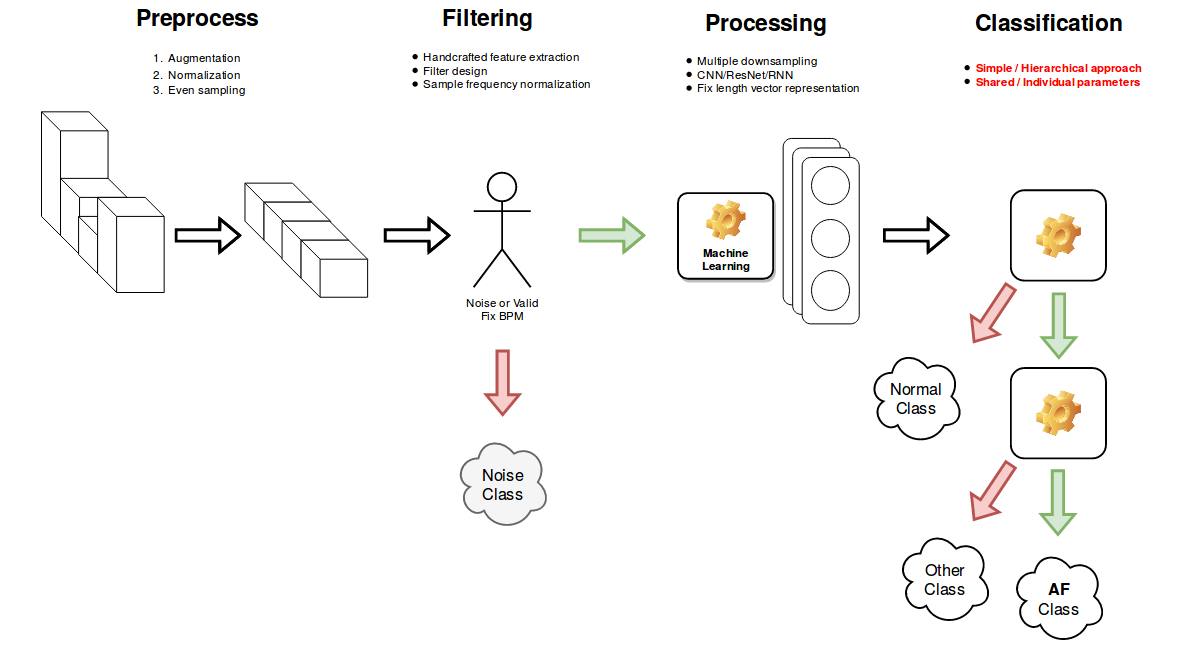
\includegraphics[width=.8\textwidth]{method}\label{fig:method}
\end{figure}

As mentioned before, we intended to exploit the late success of neural networks that offers a plenty of methods and architectures --- and a few rule of thumbs to keep in mind when preparing the blueprint.
Currently we are experimenting with hierarchical classification models.~\ref{fig:method}
At the time of writing I will describe the main building blocks we have tried before, and present the baseline our recent tests are based upon.
My role in the group is to implement and maintain the deep learning back-end, also to integrate the hand crafted features, and carry out experiments and evaluate them to determine which combination leads to the most successful architecture.

\paragraph{Variable length representation.}
First of all, we have to deal with time dependency. Since we cannot determine how long the samples will be, nor describe a time frame that would fit every relevant pattern, we have to project somehow the sample into a fixed dimensional space. In order to preserve important information by the projection we can separate samples into clusters by previously extracting features which describes best the data. These values are usually time dependent pattern fitting maps.

Fully Convolutional Network (FCN)~\cite{lecun1995convolutional, mittelman2015time}
Deep Residual Networks (ResNets) motivated by~\cite{he2016deep, wang2016time}

\paragraph{Fixed length representation.}
Once every filters have been evaluated in the end we can use different approaches: to take the wighted norm or mean of the filtered signal to represent each pattern's presence in the input signal or we can use techniques that have been proven to be successful in natural language processing tasks, the recurrent neural networks.

Long Short Term Memory network (LSTM)~\cite{hochreiter1997long, malhotra2015long}
Gated Recurrent Unit network (GRU)~\cite{chung2014empirical}

Classification:
Linear regression
Fully connected network~\cite{girshick2014rich}

?? TensorBoard/Draw.io gráftervező/PrtScr a cikkekből ??
